\begin{frame}{Taxe vs quota : curbe DM plate}

\centering
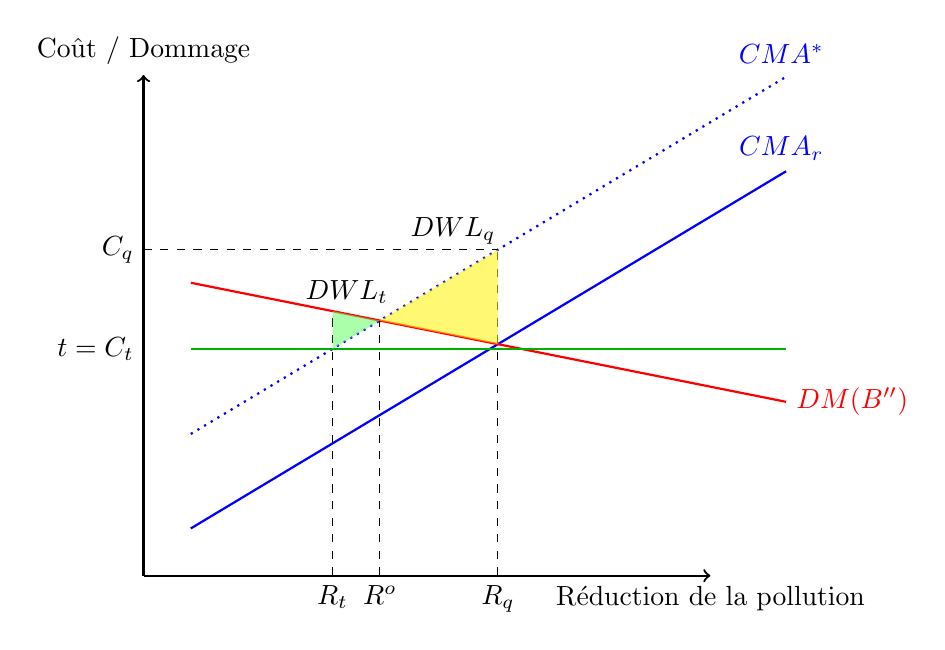
\begin{tikzpicture}[scale=1.2]

% Paramètres (MD relativement plat)
\pgfmathsetmacro{\m}{0.6}
\pgfmathsetmacro{\bE}{0.2}
\pgfmathsetmacro{\bA}{1.2}
\pgfmathsetmacro{\k}{3.2}
\pgfmathsetmacro{\d}{0.2} % MD plat

% Points clés
\pgfmathsetmacro{\Ro}{(\k-\bA)/(\m+\d)}
\pgfmathsetmacro{\yRo}{\m*\Ro+\bA}

\pgfmathsetmacro{\Rq}{(\k-\bE)/(\m+\d)}
\pgfmathsetmacro{\yRq}{\m*\Rq+\bE}

\pgfmathsetmacro{\Rt}{2.0}
\pgfmathsetmacro{\tlevel}{\m*\Rt+\bA}
\pgfmathsetmacro{\yMDatRt}{\k-\d*\Rt}

\pgfmathsetmacro{\Cq}{\m*\Rq+\bA}

% Axes
\draw[->, thick] (0,0) -- (6,0) node[below] {Réduction de la pollution};
\draw[->, thick] (0,0) -- (0,5.3) node[above] {Coût / Dommage};

% Courbes
\draw[thick, blue, dotted] (0.5, {\m*0.5+\bA}) -- (6.8, {\m*6.8+\bA});
\node[blue] at (6.75, {\m*7.2+\bA}) {$CMA^*$};

\draw[thick, blue] (0.5, {\m*0.5+\bE}) -- (6.8, {\m*6.8+\bE});
\node[blue] at (6.75, {\m*7.2+\bE}) {$CMA_r$};

\draw[thick, red] (0.5, {\k-\d*0.5}) -- (6.8, {\k-\d*6.8});
\node[red] at (7.5, {\k-\d*6.8}) {$DM (B'')$};

% Taxe
\draw[thick, green!70!black] (0.5,\tlevel) -- (6.8,\tlevel);
\node[left] at (0,\tlevel) {$t=C_t$};

% Verticales
\draw[dashed] (\Rt,0) -- (\Rt,\yMDatRt);
\node[below] at (\Rt,0) {$R_t$};

\draw[dashed] (\Ro,0) -- (\Ro,\yRo);
\node[below] at (\Ro,0) {$R^{o}$};

\draw[dashed] (\Rq,0) -- (\Rq,\Cq);
\node[below] at (\Rq,0) {$R_q$};

% Horizontale Cq
\draw[dashed] (0,\Cq) -- (\Rq,\Cq);
\node[left] at (0,\Cq) {$C_q$};

% DWL taxe
\fill[green!60, opacity=0.55]
(\Rt,\tlevel) -- (\Ro,\yRo) -- (\Rt,\yMDatRt) -- cycle;
\node at ({(\Rt+\Ro)/2 -0.1}, {\tlevel+0.6}) {$DWL_t$};

% DWL quota
\fill[yellow, opacity=0.55]
(\Ro,\yRo) -- (\Rq,\yRq) -- (\Rq,\Cq) -- cycle;
\node at ({(\Ro+\Rq)/2 +0.15}, {\yRo+0.95}) {$DWL_q$};

\end{tikzpicture}

\end{frame}


%========================
% Migration: Effect on Wages
%========================

\begin{frame}{Migration: Effect on Wages at Home}

\begin{center}
\begin{tikzpicture}[scale=0.65]
    % Original axes
    \draw[->, thick] (0,0) -- (8,0);
    \draw[->, thick] (0,0) -- (0,5) node[left] {$w$};
    
    \node[below] at (0,0) {$0_C$};
    
    % Original total labor L
    \draw[thick] (6,0) -- (6,0.1);
    \node[below] at (6,0) {$L$};
    
    % New total labor L' (after migration)
    \draw[thick, dashed] (7.5,0) -- (7.5,0.1);
    \node[below] at (7.5,0) {$L'$};
    
    % Original curves (solid)
    \draw[thick, homecolor, domain=0.5:5.5] plot (\x, {4 - 0.5*\x});
    \draw[thick, foreigncolor, domain=0.5:5.5] plot (\x, {0.5 + 0.5*\x});
    
    % Shifted food curve (after migration - measured from new L')
    \draw[thick, foreigncolor, dashed, domain=2:7] plot (\x, {-0.25 + 0.5*\x});
    
    % Original equilibrium
    \filldraw (3.5, 2.25) circle (2pt);
    \node[above left, font=\small] at (3.5, 2.25) {A};
    \draw[dashed, gray] (0, 2.25) -- (3.5, 2.25);
    \node[left, font=\small] at (0, 2.25) {$w$};
    
    % New equilibrium
    \filldraw (4.25, 1.875) circle (2pt);
    \node[above right, font=\small] at (4.25, 1.875) {B};
    \draw[dashed, gray] (0, 1.875) -- (4.25, 1.875);
    \node[left, font=\small] at (0, 1.875) {$w'$};
    
    % Arrow showing wage fall
    \draw[->, thick, gray] (-0.3, 2.25) -- (-0.3, 1.875);
    
    % Arrow showing labor increase
    \draw[->, thick, gray] (6, -0.5) -- (7.5, -0.5);
    \node[below, font=\tiny] at (6.75, -0.5) {$\Delta L$};
\end{tikzpicture}
\end{center}

\textbf{Result:} Immigration \textbf{lowers wages} in the receiving country.

\end{frame}

%========================
% Migration: Effect on Output and Specific Factors
%========================

\begin{frame}{Migration: Effect on Output and Returns}

\textbf{At Home (receiving country), after immigration:}

\vspace{0.3cm}

\begin{itemize}
    \item $L \uparrow$ $\Rightarrow$ Output in \textbf{both} sectors increases
    
    \vspace{0.2cm}
    
    \item Wages fall: $w \downarrow$
    
    \vspace{0.2cm}
    
    \item \textbf{Returns to capital and land increase:}
    \begin{itemize}
        \item Method 1: Revenue $-$ Labor costs = Higher profits (wages fell)
        \item Method 2: $MPK \uparrow$ and $MPT \uparrow$ (more workers per machine/acre)
    \end{itemize}
\end{itemize}

\vspace{0.5cm}

\textbf{Summary of immigration effects:}
\begin{itemize}
    \item \textcolor{laborcolor}{Workers (native):} \textbf{Lose} (wages fall)
    \item \textcolor{capitalcolor}{Capital owners:} \textbf{Gain}
    \item \textcolor{landcolor}{Landowners:} \textbf{Gain}
\end{itemize}

\end{frame}

%========================
% Migration: PPF Expansion
%========================

\begin{frame}{Migration: Effect on the PPF}

\begin{columns}[T]
\begin{column}{0.55\textwidth}
\centering
\begin{tikzpicture}[scale=0.6]
    % Axes
    \draw[->, thick] (0,0) -- (7,0) node[below] {$Q_C$};
    \draw[->, thick] (0,0) -- (0,6) node[left] {$Q_F$};
    
    % Original PPF
    \draw[thick, myblue, domain=0:5] plot ({4.5*cos(\x*18)}, {4.5*sin(90-\x*18)});
    \node[myblue, left] at (3.5, 2.5) {PP};
    
    % Expanded PPF (after immigration)
    \draw[thick, myblue, dashed, domain=0:5] plot ({5.5*cos(\x*18)}, {5.5*sin(90-\x*18)});
    \node[myblue, right] at (5, 3) {PP'};
    
    % Arrow showing expansion
    \draw[->, thick, gray] (3.2, 3.2) -- (3.9, 3.9);
\end{tikzpicture}
\end{column}

\begin{column}{0.45\textwidth}
\textbf{Immigration expands the PPF}

\vspace{0.3cm}

More labor $\Rightarrow$ More output possible in \textbf{both} sectors

\vspace{0.3cm}

\textbf{Question:} How can you see in the PPF that labor mobility and international trade are potential \textbf{substitutes}?

\vspace{0.3cm}

\onslide<2->{
\textit{Both expand consumption possibilities beyond autarky PPF}
}
\end{column}
\end{columns}

\end{frame}

%========================
% FDI: Setup
%========================

\begin{frame}{FDI in the Specific Factors Model}

\textbf{Setup:} Capital flows from Foreign to Home (FDI inflow).

\vspace{0.3cm}

\textbf{At Home (receiving country):}
\begin{itemize}
    \item Increase in capital stock: $K \uparrow$
    \item Labor and land unchanged
\end{itemize}

\vspace{0.3cm}

\textbf{Question:} What happens to wages and returns to specific factors?

\end{frame}

%========================
% FDI: Effects
%========================

\begin{frame}{FDI: Effect on Wages and Returns}

\textbf{When capital increases in Home:}

\vspace{0.3cm}

\begin{itemize}
    \item \textbf{Cloth sector expands} (uses more capital)
    
    \vspace{0.2cm}
    
    \item Labor shifts toward cloth: $L_C \uparrow$, $L_F \downarrow$
    
    \vspace{0.2cm}
    
    \item \textbf{Wages rise:} $w \uparrow$
    \begin{itemize}
        \item More capital per worker in cloth $\Rightarrow$ higher $MPL_C$
    \end{itemize}
\end{itemize}

\vspace{0.3cm}

\textbf{Returns to specific factors:}
\begin{itemize}
    \item \textcolor{capitalcolor}{Rental on capital ($R_K$):} \textbf{Falls} (diminishing returns to capital)
    \item \textcolor{landcolor}{Rental on land ($R_T$):} \textbf{Falls} (labor leaves agriculture)
\end{itemize}

\vspace{0.3cm}

\textbf{Summary:} Workers gain, owners of specific factors lose.

\end{frame}

%========================
% FDI: PPF Effect
%========================

\begin{frame}{FDI: Effect on the PPF}

\begin{columns}[T]
\begin{column}{0.55\textwidth}
\centering
\begin{tikzpicture}[scale=0.6]
    % Axes
    \draw[->, thick] (0,0) -- (7,0) node[below] {$Q_C$};
    \draw[->, thick] (0,0) -- (0,6) node[left] {$Q_F$};
    
    % Original PPF
    \draw[thick, myblue, domain=0:5] plot ({4.5*cos(\x*18)}, {4.5*sin(90-\x*18)});
    
    % Biased expansion (more in cloth direction)
    \draw[thick, myblue, dashed, domain=0:5] plot ({5.5*cos(\x*18)}, {4.5*sin(90-\x*18)});
    
    % Labels
    \node[myblue, left] at (2.5, 4) {PP};
    \node[myblue, right] at (5.2, 2.5) {PP'};
    
    % Arrow showing biased expansion
    \draw[->, thick, gray] (4, 2.5) -- (5, 2.5);
\end{tikzpicture}
\end{column}

\begin{column}{0.45\textwidth}
\textbf{FDI causes biased expansion}

\vspace{0.3cm}

Capital is specific to cloth $\Rightarrow$ PPF expands more in cloth direction

\vspace{0.3cm}

\textbf{Compare to immigration:}
\begin{itemize}
    \item Immigration: symmetric expansion
    \item FDI: biased toward capital-using sector
\end{itemize}
\end{column}
\end{columns}

\end{frame}

%========================
% Gains from Factor Flows
%========================

\begin{frame}{Gains from Labor and Capital Flows}

\textbf{Question:} Where do the gains come from for the country that \textbf{sends} capital or workers?

\vspace{0.3cm}

\textbf{Sending country gains from:}

\begin{itemize}
    \item \textbf{Remittances} (migration): Workers send money home
    
    \vspace{0.2cm}
    
    \item \textbf{Return on capital} (FDI): Profits repatriated to home country
    
    \vspace{0.2cm}
    
    \item \textbf{Higher returns abroad:} Factors earn more in destination country (where they were scarce)
\end{itemize}

\vspace{0.3cm}

\textbf{World gains:}
\begin{itemize}
    \item Total world output increases when factors move to where they are more productive
    \item Similar logic to gains from trade in goods
\end{itemize}

\end{frame}